\documentclass[12pt,letterpaper]{article}


\usepackage{dcolumn}% Align table columns on decimal point
\usepackage{bm}% bold math
%
%Paquete de Idioma
\usepackage[spanish]{babel}
%
%Codificación Alfabeto
\usepackage[utf8]{inputenc}
%
%Codificación de Fuente
\usepackage[T1]{fontenc}
%
%Índice
\usepackage{makeidx}
%
%Gráficos
\usepackage{graphicx}
\usepackage{subfig}
%\usepackage{xcolor}
%
%Matemática
\usepackage{amsmath}
\usepackage{amsfonts}
\usepackage{amssymb}
%\usepackage{amstext}
%
%Estilo de Página Numeración superior
%\pagestyle{headings}
%
%Hiperlinks \href{url}{text}
\usepackage[pdftex]{hyperref}
%
%Graficos y tablas
\usepackage{multirow}
%\usepackage{multicol}

%El paquete float es importante para las imágenes con la opción [H] para que las imágenes se coloquen en donde lo deseamos
\usepackage{float}
\usepackage{booktabs}
%
\decimalpoint
%\bibliographystyle{IEEEtran}
%\bibliography{IEEEabrv,mybibfile}
%Para tachar dimencionales
\usepackage{cancel}
%
%%<<<<<<<<<<<<<<<<<<<<  >>>>>>>>>>>>>>>>>>>
%<<<<<<<<<<<<<<<<<<<<  >>>>>>>>>>>>>>>>>>>
%<<<<<<<<<<<<<<<<<<<<  >>>>>>>>>>>>>>>>>>>
%	  Paquetes agregados al formato
%<<<<<<<<<<<<<<<<<<<<  >>>>>>>>>>>>>>>>>>>
%<<<<<<<<<<<<<<<<<<<<  >>>>>>>>>>>>>>>>>>>
%<<<<<<<<<<<<<<<<<<<<  >>>>>>>>>>>>>>>>>>>


%<<<<<<<<< Comando valores absolutos |x| >>>>>
\newcommand{\abs}[1]{\lvert1\rvert}
%<<<<<<<<< Comando para la normal ||x|| >>>>>
\newcommand{\norm}[1]{\lVert1\rVert}

%<<<<<<<<< para saltos de página usar  \clearpage >>>>>
%<<<<<<<<< para saltos entre líneas usar \vspace{2cm}>>>>>
%<<<<<<<<< para espaciado horizontal \hspace{1cm}>>>>>
%<<<<<<<<< para colocar url o referencias a url usar \url{http://www.latex-project.org/} o  \href{http://www.latex-project.org/}{latex project}>>>>>>>

%<<<<<<<<<<<<<<<<<<<<  >>>>>>>>>>>>>>>>>>>

%Paquete para configurar medidas de las tablas
\usepackage{tabularx}
%Forma del comando
%\begin{tabular}{|m{0.22\linewidth}|m{0.22\linewidth}|}


%<<<<<<<<< Para configurar \begin{enumerate}[A)]  en donde está la letra "A" escogemos como queremos enumerar, ejemplo \begin{enumerate}[i)]>>>>>>>>>>>>>>

\usepackage{enumerate}

%<<<<<<<<< Cambiar columnas >>>>>

%Se aconseja colocar el documento a una columna y luego cambiarle con forme se vaya utilizando. comandos:
%\begin{multicols}{2}
	%contenido
%\end{multicols}
\usepackage{multicol} %Paquete cambiar columnas

%<<<<<<<<<<<<<<<<<<<<  >>>>>>>>>>>>>>>>>>>

%Configurar sangría
\setlength{\parindent}{0pt}

%>>>>>>>>>>>>>>>>>>Esto es para interlineado V2<<<<<<<

%Para interlineado
%\renewcommand{\baselinestretch}{1.5}

%Para cambiar la sangría 2
%\setlength{\parindent}{4em}

%Espaciado entre parrafos
%\setlength{\parskip}{1em}

%<<<<<<<<<<<<<<<<<<<<  >>>>>>>>>>>>>>>>>>>

%Para colocar punto decimal en lugar de coma automático.
\spanishdecimal{.}

%Para colocar anotaciónes al pié de página, podemos utilizar \footnote{Anotación pié de página}, pegado a la palabra a la cuál se hará la anotación.

%<<<<<<<<<<<<<<<<<<<<  >>>>>>>>>>>>>>>>>>>

%Para agregar un índice: \tableofcontents



%<<<<<<<<<<<<<<<<<<<<  >>>>>>>>>>>>>>>>>>>

% El comando \ balance se puede utilizar para equilibrar las columnas en la página final si se desea. Debe colocarse en cualquier lugar dentro de la primera columna de la última página.
\usepackage{balance}

%\balance
%<<<<<<<<<<<<<<<<<<<<  >>>>>>>>>>>>>>>>>>>

%Use el paquete pdfpages.
%Para incluir todas las páginas en el archivo PDF:
% \includepdf[pages=-]{myfile.pdf}

%Para incluir solo la primera página de un PDF:
%\includepdf[pages={1}]{myfile.pdf}

%Ejecute texdoc pdfpages en un Shell para ver el manual completo de pdfpages.

\usepackage{pdfpages}



%<<<<<<<<<<<<<<<<<<<<  >>>>>>>>>>>>>>>>>>>

%Este comando sirve para importar archivos txt.

\usepackage{verbatim}

% Usar \verbatiminput{archivo.tex}

\usepackage{listings}

%<<<<<<<<<<<<<<<<<<<<  >>>>>>>>>>>>>>>>>>>
%Para agregar una caratula más personalizada
%\begin{titlepage}
%	*
%\begin{titlepage}

%<<<<<<<<<<<<<<<<<<<<  >>>>>>>>>>>>>>>>>>>

%Para agregar texto entre ecuaciónes
%\textup{•}
%<<<<<<<<< Permite poner varios autores >>>>>>>>>>>>>

\usepackage{authblk}

%\author[1]{Author \thanks{correo1•university.edu}}
%\author[1]{Author \thanks{correo2•university.edu}}
%\author[1]{Author \thanks{correo3•university.edu}}
%\author[2]{Author \thanks{correo3•university.edu}}
%\author[2]{Author %\thanks{correo4•university.edu}}

%\affil[1]{Department of Computer Science, \LaTeX\ University}
%\affil[2]{Department of Mechanical Engineering, \LaTeX\ University}

%<<<<<<<<<<<<<<<<<<<<  >>>>>>>>>>>>>>>>>>>

%Este comando sirve para importar archivos txt.

\usepackage{verbatim}

\usepackage{listings}

%<<<<<<<<<<<<<<<<<<<<  >>>>>>>>>>>>>>>>>>>
%<<<<<<<<<<<<<<<<<<<<  >>>>>>>>>>>>>>>>>>>


\usepackage[left=1.5cm,right=1.5cm,top=1.5cm,bottom=1.5cm]{geometry}
\author{Héctor Fernando Carrera Soto \\
 Carné: 201700923}
\title{Comandos para usar Django}
\date{20 de marzo de 2022}

\begin{document}

%%%%%%%%%%%%%%%%%
%	Encabezado	%
%%%%%%%%%%%%%%%%%


\maketitle

%%%%%%%%%%%%%%%%%%%%%%%%%
%	Creando proyecto	%
%%%%%%%%%%%%%%%%%%%%%%%%%

\section{Creando un proyecto de Django}

Para realizar un proyecto django, nos dirigimos a cualquier carpeta en el que lo almacenaremos, nos dirigimos a la ruta creada desde la termina, en windows o linux y escribimos el siguiente comando:\\

\textbf{\emph{\$ django-admin startproject [Nombre\_del\_proyecto]}}\\

Luego verificamos que todo se encuentre correcto, ejecutando nuestro \emph{manage.py} creado por el comando anterior, escribiendo el siguiente comando:\\

\textbf{\emph{\$ python manage.py runserver}}\\

Copiamos la dirección mostrada en nuestro navegador web:\\

\textbf{\emph{\$ Starting development server at http://127.0.0.1:8000/
}}\\

si vemos la siguiente página, figura \ref{fig_pantalla_inicio}, es porque todo está bien con nuestro paquete Django.\\

\begin{figure}[H]
\centering
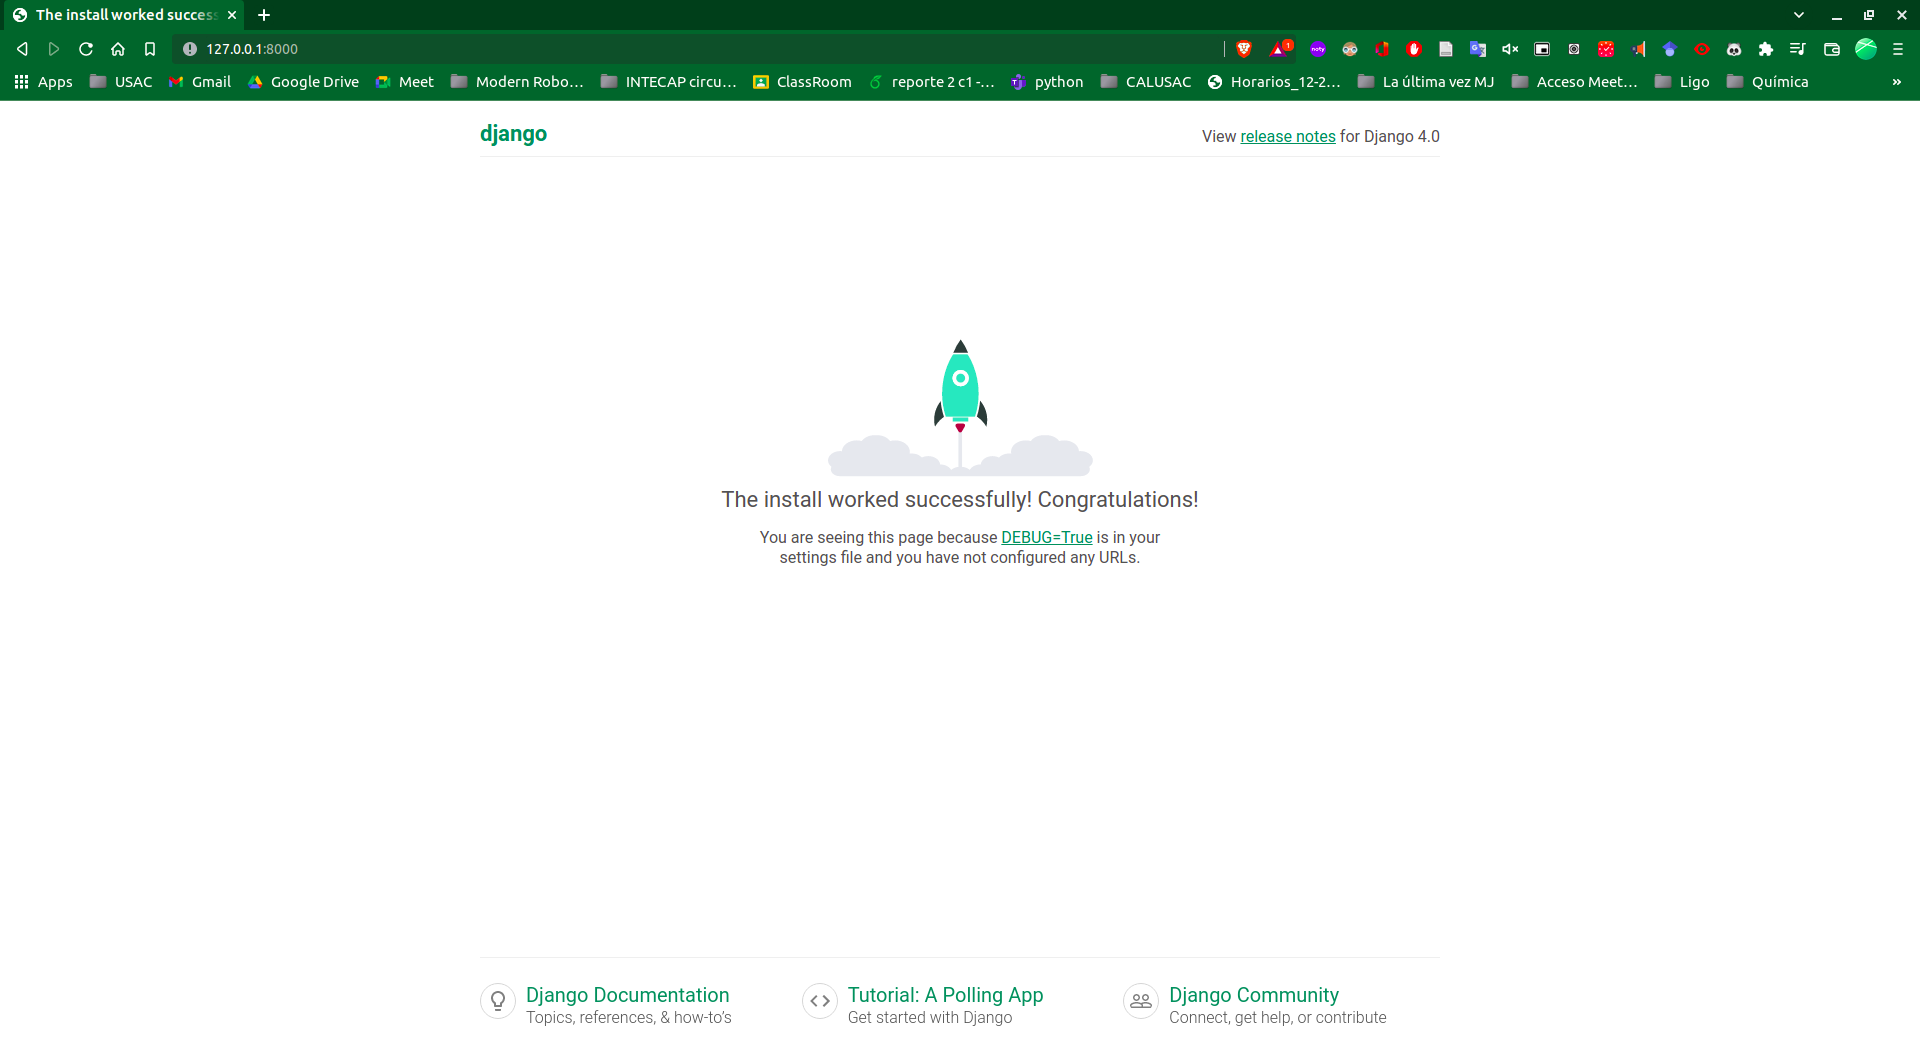
\includegraphics[scale=0.2]{pantalla_inicio.png}
\caption{Elaboracón propia.}
\label{fig_pantalla_inicio}
\end{figure}

%%%%%%%%%%%%%%%%%%%%%
%	Creando página	%
%%%%%%%%%%%%%%%%%%%%%

\section{Creando una página}

Creamos un archivo \emph{views.py} en la carpeta contenedora, afuera de la carpeta \emph{\_\_pycache\_\_}.\\

Agregamos el siguiente código:\\



\lstset{language=python, breaklines=true, basicstyle=\footnotesize}
\begin{lstlisting}[frame=single]

from django.http import HttpResponse

def saludo(request): \# Primera vista
    return HttpResponse(''Hola mundo!'')

\end{lstlisting}




Luego nos dirigimos a nuestro archivo \emph{urls.py} y agregamos la siguiente línea de código dentro de la tupla en \emph{urlpatterns}:




\lstset{language=python, breaklines=true, basicstyle=\footnotesize}
\begin{lstlisting}[frame=single]

path('saludo/', saludo), #Saludo/ puede ser diferente

\end{lstlisting}

Quedando el código de la siguiente forma:\\

\lstset{language=python, breaklines=true, basicstyle=\footnotesize}
\begin{lstlisting}[frame=single]

from django.contrib import admin
from django.urls import path
from Albergue_mascotas.views import saludo

urlpatterns = [
    path('admin/', admin.site.urls),
    path('saludo/', saludo), #Saludo/ puede ser diferente
]

\end{lstlisting}

\section{Primeras configuraciónes}

Para crear las primera configuraciones de \emph{migrate} utlizamos el siguiente comando en la carpeta en el que tenemos el archivo \emph{manage.py}:\\

\begin{verbatim}
$ python manage.py migrate
\end{verbatim}

\section{Superusuario}

También crearemos un super usuario para que podamos agregar o designar a una persona como administrador de toda la página con el siguiente comando en la terminal:\\

\begin{verbatim}
$ python manage.py createsuperuser
\end{verbatim}

y tendremos que ingresar los siguientes datos:\\

\begin{verbatim}
Username (leave blank to use 'hefecaso'): fernando
Email address: admin@admin.com
Password:
Password (again):
This password is too short. It must contain at least 8 characters.
Bypass password validation and create user anyway? [y/N]: y
Superuser created successfully.
\end{verbatim}


\end{document}
